%DIF PREAMBLE EXTENSION ADDED BY LATEXDIFF
%DIF UNDERLINE PREAMBLE %DIF PREAMBLE
\RequirePackage[normalem]{ulem} %DIF PREAMBLE
\RequirePackage{color}\definecolor{RED}{rgb}{1,0,0}\definecolor{BLUE}{rgb}{0,0,1} %DIF PREAMBLE
\providecommand{\DIFadd}[1]{{\protect\color{blue}\uwave{#1}}} %DIF PREAMBLE
\providecommand{\DIFdel}[1]{{\protect\color{red}\sout{#1}}}                      %DIF PREAMBLE
%DIF SAFE PREAMBLE %DIF PREAMBLE
\providecommand{\DIFaddbegin}{} %DIF PREAMBLE
\providecommand{\DIFaddend}{} %DIF PREAMBLE
\providecommand{\DIFdelbegin}{} %DIF PREAMBLE
\providecommand{\DIFdelend}{} %DIF PREAMBLE
%DIF FLOATSAFE PREAMBLE %DIF PREAMBLE
\providecommand{\DIFaddFL}[1]{\DIFadd{#1}} %DIF PREAMBLE
\providecommand{\DIFdelFL}[1]{\DIFdel{#1}} %DIF PREAMBLE
\providecommand{\DIFaddbeginFL}{} %DIF PREAMBLE
\providecommand{\DIFaddendFL}{} %DIF PREAMBLE
\providecommand{\DIFdelbeginFL}{} %DIF PREAMBLE
\providecommand{\DIFdelendFL}{} %DIF PREAMBLE
%DIF END PREAMBLE EXTENSION ADDED BY LATEXDIFF

% \date{} % \vspace*{-0.2in}}

\documentclass[10pt,preprint]{sigplanconf} % SIGPLAN

\nocaptionrule

% USENIX
%\usepackage{mathptmx} % rm & math
\usepackage[scaled=0.90]{helvet} % ss
\usepackage{courier} % tt
\normalfont
\usepackage[T1]{fontenc}

% \usepackage{lmodern}
% \usepackage{times}
\usepackage{subfigure}
\usepackage{url}
\urlstyle{rm}
\usepackage[
      colorlinks=false,    %no frame around URL
      urlcolor=black,    %no colors
      menucolor=black,    %no colors
      linkcolor=black,    %no colors
      pagecolor=black,    %no colors
]{hyperref}

\usepackage{color}
\usepackage{listings}
\usepackage{amsmath}
\usepackage{amsfonts}
\usepackage{amssymb}
\usepackage{comment} 
\usepackage{setspace}
\singlespacing
%\onehalfspacing
\newtheorem{thm}{Theorem}
\newtheorem{prop}[thm]{Proposition}
\newtheorem{cor}[thm]{Corollary}
\newtheorem{lem}[thm]{Lemma}
\newtheorem{defn}[thm]{Definition}

\newcommand{\cfunction}[1]{{\bf \tt #1}}
\newcommand{\malloc}{\cfunction{malloc}}
\newcommand{\realloc}{\cfunction{realloc}}
\newcommand{\free}{\cfunction{free}}
\newcommand{\madvise}{\cfunction{madvise}}
\newcommand{\brk}{\cfunction{brk}}
\newcommand{\sbrk}{\cfunction{sbrk}}
\newcommand{\mmap}{\cfunction{mmap}}
\newcommand{\munmap}{\cfunction{munmap}}
\newcommand{\mprotect}{\cfunction{mprotect}}
\newcommand{\mlock}{\cfunction{mlock}}

\hyphenation{app-li-ca-tion}
\hyphenation{Die-Hard}
\hyphenation{Ar-chi-pe-la-go}
\hyphenation{buf-fer}

\lstset{language=c++, basicstyle=\ttfamily\scriptsize,frame=trbl,tabsize=4,numbers=left,numberstyle=\tiny}

\definecolor{Gray}{cmyk}{0,0,0,0.5}
\newcommand{\footnotenonumber}[1]{{\def\thempfn{}\footnotetext{\small #1}}}

%\usepackage{usenix,epsfig,endnotes}
\usepackage{subfigure}
\usepackage{url}
% \usepackage{breakurl}
\urlstyle{rm}
\usepackage[
      colorlinks=false,    %no frame around URL
      urlcolor=black,    %no colors
      menucolor=black,    %no colors
      linkcolor=black,    %no colors
      pagecolor=black,    %no colors
]{hyperref}

\usepackage{subfigure}
\usepackage{color}
\usepackage{listings}
\usepackage{amsmath}
\usepackage{amsfonts}
\usepackage{amssymb}
\usepackage{comment} 
\usepackage{setspace}
\usepackage{graphicx}
\newcommand{\sheriff}{\textsc{Sheriff}}
\newcommand{\sheriffprotect}{\textsc{FS-Patrol}}
\newcommand{\sheriffdetect}{\textsc{FS-Detective}}
\newcommand{\pthreads}{\texttt{pthreads}}

\lstdefinelanguage{c++threads}[]{c++}{morekeywords={pthread_create,pthread_join}}
\lstset{language=c++threads, basicstyle=\ttfamily\scriptsize,frame=trbl,tabsize=4} % ,numbers=left,numberstyle=\tiny}


\begin{document}

\conferenceinfo{OOPSLA 2011}

% Sheriff: Efficient and Precise False Sharing Detection
\title{Precise Detection and Automatic Mitigation of False Sharing}

\authorinfo{Tongping~Liu \and Emery~D.~Berger}
{Department of Computer Science \\
University of Massachusetts, Amherst \\
Amherst, MA 01003}
{\{tonyliu,emery\}@cs.umass.edu}

\maketitle

\begin{abstract}
%How is existing work?
%Sharing inside mulithreaading programs is not easy, they can easily cause correctness or performance problem. 
%Inappropriate sharing can dramatically degrade the performance of 
%mulithreading programs and seriously affect the scalability. 
%So detecting false sharing accurately and precisely can be helpful for user to fix corresponding performance problem. 

\begin{comment}
False sharing is notorious for performance degradation in multithreaded
programs. It apprears when two or more threads running on different cores periodically access 
different portions of data that can fit into one cache line. Since caching
system in a multicore processor needs to ensure a coherent view of memory
accross all cores, it has to grant an exclusive access
for each write operation by invidating duplicate copies in other cores. As a
result, frequent cache invalidation can seriously affect the scalability and
performance of multithreaded programs.
\end{comment} 

False sharing is a notorious performance issue for different software stacks, 
which can dramatically degrade the performance and seriously affect the scalability of 
systems.

%Many reserach efforts have been made to detect false sharing. 
Unfortunately, previous approaches to detect false sharing
either introduce significant performance overhead, or fail
to report false sharing accurately and precisely, or have different limitations of usage. 
%\sheriff{}, the prior state-of-the-art tool, 
%can only detect write-write false sharing in applications using \pthreads{} library.
This paper presents a novel approach, \Predator{}, to combine compiler instrumentation
and runtime system to detect false sharing. 
%the compiler instruments every memory access and 
%the runtime system collects and analyzes memory accesses to detect false sharing problems.
Since it does not rely on any hardware, OS or threading library, this approach can be
applied to the entire software stack without any limitation. 
\Predator{} can detect false sharing accurately and precisely: it reports no 
false positives and pinpoints exact objects with false sharing problems.
%Also, unlike previous work, this method can be extended to
%identify false sharing problems across the entire software stack, including 
%hypervisors, operating systems, libraries and applications. 
Experimental results on two popular benchmark suites 
show that \Predator{} not only detected all known false sharing problems but also revealed 
two unknown false sharing problems.
Besides, \Predator{} have successfully detected false sharing of real applications,
including \texttt{mysql} server application and \texttt{boost} library. Fixing these
false sharing problems improves performance by $6\times$ and $40\%$ correspondingly.

Moreover, existing tools can only detect those manifested false sharing problems.
However, occurrences of false sharing can be affected by alignments between
objects and cache lines: any change of compiler optimization, compiler, memory manager, 
memory allocation order, cache line size or different target binary 
may change alignments, and thus affect occurrences of false sharing, 
which leaves many of them undetected by existing tools.
\Predator{} is the first tool which can accurately predict possible false sharing 
without the need of occurrences. 
It can report all false sharing problems with only one execution and with reasonable overhead, 
around $6.7\times$ performance overhead on average.

%What is novel in our work?
%How is the performance overhead?

\end{abstract}

%\terms
%Performance, False sharing

%\keywords
%Concurrency, False Sharing, Performance, Multi-threaded program

%%%%%%%%%%%%%%%%%%%%%%%%%%%%%%%%%%%%%%%%%%%%%%%%%%%%%%%%%%%%%%%%%%%%%%%%%%%%%%%%%%%%%%%%%%%%%
%%%%%%%%%%%%%%%%%%%%%%%%%%%%%%%%%%%%%%%%%%%%%%%%%%%%%%%%%%%%%%%%%%%%%%%%%%%%%%%%%%%%%%%%%%%%%

\section{Introduction}
%False sharing problem is a cache usage problem. 
%Cache, with much faster access speed than main memory, is normally utilized by CPU
%to accelerate program executions by preloading a fixed size of data into the cache each time, 
%called as a cache line.  

%%%%%%%%%%%%%%%%%%%%%%%%%%%%%%%%%%%%%%%%
% Why 
%%%%%%%%%%%%%%%%%%%%%%%%%%%%%%%%%%%%%%%%
\label{sec:intro} 
False sharing is notorious for performance degradation in multithreaded
programs due to cache coherence protocol, which exists in most mordern 
 mutlicore processors.
The reason of having cache coherence protocol is to ensure the correctness of
program executions: 
if some cache line data on a core needs to be updated, the duplicated data in any other core's private 
cache must be invalidated at cache-line level (e.g., 64 Bytes). 
However, frequent invalidations can cause severe performance problem.
In the case of false sharing where multiple threads access different locations
in the same cache line in a \textit{ping-pong} manner, generated cache
invalidations can easily degrade program performance as much as an order of magnitude. 
%Because cache invalidation can cause a thread accessing the same cache line to stall and wait for the data 
%to be loaded from main memory, wasting both the CPU time and memory bandwidth in the same time. 
Unfortunately, the hardware evolution is on the venue of building more cores
with larger cache line size, which makes false sharing increasingly common.

Prior studies have shown that false sharing affects different levels of current software stack.
It has been found in OS (Linux kernel~\cite{OSfalsesharing}), Java virtual machine~\cite{JVMfalsesharing}, 
common libraries~\cite{libfalsesharing} and real applications~\cite{appfalsesharing, mysql}. 
People also observed false sharing in runtime system such as share memory system
~\cite{dsmfalsesharing} and transactional memory ~\cite{tmfalsesharing}.
Although many efforts have been made in false sharing detection, existing
tools have various limitations:
they either introduce significant performance overhead~
\cite{falseshare:simulator, falseshare:binaryinstrumentation1,falseshare:binaryinstrumentation2}, or 
 are incapable of reporting false sharing 
precisely and accurately~\cite{qinzhaodetection, detect:ptu, detect:intel, falseshare:binaryinstrumentation1, DProf, falseshare:binaryinstrumentation2}, 
or require special OS support~\cite{OSdetection}.
% or they can only detect one kind of
%false sharing problem on a specific multithreading library~\cite{sheriff}.
The state-of-the-art tool, Sheriff~\cite{sheriff} overcomes these limitations. However, 
it can only detect write-write type false sharing in programs using pthreads library,
and can not work correctly on programs using ad-hoc synchronizations or using stack variables to 
communicate among different threads. Also, to the best of our knowledge, none of them has been 
utilized to find false sharing problem in real applications.

Despite their different features and limitations, all existing detection tools 
have two common drawbacks.
The first drawback is that existing techniques can not detect false sharing for 
the entire software stack, whereas they can work on a specific level of software stack.
The second drawback is that they can only detect those false sharing occurring in current execution.
However, as pointed out by Nanavati et al.~\cite{OSdetection}, 
some dynamic properties of a system can easily 
change the manifest of false sharing problems. They also give an example that 
{\it "GCC fixes false sharing in the Phoenix linear\_regression benchmark 
at -O2 and -O3 optimization, while clang fails to even at the highest
optimization level".}
To our understanding, those dynamic properties include 
choosing different compiler, 
enabling different compiler optimizations, 
using different memory management schemes,
and changing different target platforms such as address mode (32-bit or 64-bit) and cache line
size (64 Bytes or 128 Bytes) and so on. Unfortuantely, 
existing detection tools do not consider these dynamic properties, and
therefore are unable to identify potential performance-degrading false
sharing problems that may occur in an execution under a set of different 
dynamic properties.

In this paper, we propose a new false sharing detector, \defaults{}, aiming to
not only {\it detect} all existing false sharing problems accurately and precisely,
but {\it predict} those potential 
false sharing problems that may appear in a slightly different environment. 
%To be more specific, 
%\defaults{} can report potential false sharing problems with different cache line size and different starting address of an object 
%without the need of another execution. 

\Defaults{} has the following contributions:
\begin{itemize}
\item
% methodology
\defaults{} provides a novel false sharing detection method by
combining compiler instrumentation with runtime system.
%, which can avoid the shortcomings of existing tools. 
Since \defaults{} neither relies on the support of specific hardware and OS ,
nor binds to specific threading library, 
it is suitable for the entire software stack, 
i.e., hypervisors, operating systems, libraries and applications. 
%Since compiler can be utilized to do selective instrumentation, 
%\defaults{} can be utilized to detect all kinds of false sharing problem with ideal overhead. 

% effect: can detect all kinds of false sharing problems.
\item
\defaults{} can actually detect all kinds of false sharing problems accurately and precisely 
with reasonable overhead. 
It reveals some unknown false sharing problems in those benchmark suites evaluated by 
previous approaches.
It is also the first tool to detect false sharing problems existing in real applications, e.g.,
\texttt{mysql} server application and \texttt{boost} library.
% combine compiler instrumentation with runtime system, so that it can 
%detect all kinds of false sharing problem including write-write false sharing. 
%avoid the shortcomings of runtime-only system, where Sheriff can not detect the read-writee false sharings. 
%Also, because of the limit of their implementation, Sheriff can not support the program using the ad hoc synchronization
%or using the stack variables to communicate among different threads.
%Also, it looks like that we can provide a evenly performance overhead.
%Also, sheriff should only work on specific thread library, currently, it can only work on pthreads library. 
%We are trying to extending the same idea to different thread library. Now we can also run DeFault to detect all 
%false sharings using other threads libraries.

% prediction
\item
\defaults{} is the first approach to predict potential false sharing that does
not manifest in an execution but may appear and greatly affect the performance of programs 
in a slightly different environment. 
This avoids the predicament of detection tools: problems may occur in a real
environment rather than test environment due to environmental changes. 
%Existing approaches is based on specific hardware,
%runtime environment(using specific libraries and compilers) and specific cache line size, which is OK to detect those 
%existing false sharings. But they fail to capture those variables or objects which can greately slow down performance 

%In order to save memory usage, we propose a threshold invoked detection based on the predefined number of writes on a cache line, which
%can be used to track the .

\end{itemize}

The orgnization of this paper is as follows .....

%There are two types of false sharings:
%A. Different threads are accessed different locations according to the definition of flase sahrings. 
%B. Locations with a large amount of reads is placed in the cache line with a large amount of writes.
%For the second type, existing tools may tend to miss that.  


\section{Related Work}
\label{sec:relatedwork}

This section describes related work in false sharing detection, prevention, or both; no prior work predicts false sharing.

\subsection{False Sharing Detection}
Schindewolf et al.\ designed a tool based on the SIMICS functional simulator to report different kinds of cache usage information, such as cache misses and cache invalidations~\cite{falseshare:simulator}. Pluto relies on the Valgrind dynamic instrumentation framework to track the sequence of memory read and write events on different threads, and reports a worst-case estimation of possible false sharing~\cite{falseshare:binaryinstrumentation1}.
Similarly, Liu uses Pin to collect memory access information, and reports total cache miss information~\cite{falseshare:binaryinstrumentation2}.
These tools impose about $100-200\times$ performance overhead.

Zhao et al.\ present a tool based on the DynamoRIO framework to detect false sharing and other cache contention problems
for multithreading programs~\cite{qinzhaodetection}. 
It uses a shadow memory technique to maintain memory access history and detects cache invalidations based on the ownership of cache lines. However, it can only support at most $8$ threads. In addition, it cannot differentiate cold cache misses from actual false sharing problems.

Intel's performance tuning utility (PTU) uses Precise Event Based Sampling (PEBS) hardware support to detect false sharing problems~\cite{detect:ptu,detect:intel}.  PTU cannot distinguish true sharing from false sharing. In addition, PTU aggregates memory accesses without considering memory reuse and access interleavings, leading to numerous false positives. Sanath et al.\ designed a machine learning based approach to detect false sharing problems. They train their classifier on mini-programs and apply this classifier to general programs~\cite{mldetect}. Instead of instrumenting memory accesses, this tool relies on hardware performance counters to collect memory accesses events. This approach operates with extremely low overhead but ties false sharing detection to a specific hardware platform.

In addition to their individual disadvantages,
all approaches discussed above share a common shortcoming:  
they cannot pinpoint the exact location of false sharing in the source code, so programmers must manually examine the source code to identify problems.

Pesterev et al.\ present DProf, a tool that help programmers identify cache misses based on AMD's instruction-based sampling hardware~\cite{DProf}. DProf requires manual annotation to locate data types and object fields, and cannot detect false sharing when multiple objects reside on the same cache line.

\subsection{False Sharing Prevention}

Jeremiassen and Eggers use a compiler transformation to automatically adjust the memory layout of applications through padding and alignment~cite{falseshare:compile}. Chow et al.\ alter parallel loop scheduling in order to avoid false
sharing~\cite{falseshare:schedule}. These approaches only works for regular, array-based scientific code.

Berger et al.\ describe Hoard, a scalable memory allocator that can reduce the possibility of false sharing by making different threads use different heaps~\cite{Hoard}. Hoard cannot avoid false sharing problem in global variables or within a single heap object: the latter appears to be the primary source of false sharing problems.

\subsection{False Sharing Detection and Prevention}

\sheriff{} provides two tools to handle false sharing based on its ``threads-as-processes'' framework~\cite{sheriff}.
\Sheriff{}'s detection tool reports false sharing accurately and precisely with only $20\%$ performance overhead.
However, it can only detect write-write false sharing, and only works for programs that use the \pthreads{} library. It can also break programs that communicate across different threads with stack variables or \emph{ad hoc} synchronizations. These shortcomings limit \Sheriff{}'s usefulness for real-world applications.  
\Predator{} can detect all kinds of false sharing and imposes no limitations on the kind of applications it works on. 

\Sheriff{}'s prevention tool prevents false sharing altogether, eliminating the need for programmer intervention. However, in programs with many synchronization calls, the overhead imposed by \Sheriff{} could lead to performance degradation.

Plastic leverages the sub-page granularity memory remapping facility provided by the Xen hypervisor to detect and tolerate false sharing automatically~\cite{OSdetection}. However, the sub-page memory remapping mechanism is not currently supported by most existing operating systems, reducing its generality. In addition, Plastic cannot pinpoint the exact source of false sharing.  
In order to utilize Plastic's prevention tool, a program has to run on the Xen hypervisor, limiting the applicability of their prevention technique.


\section{\sheriff{}}
\label{sec:simulation}


\sheriff{} is a functional replacement for the \pthreads{} library
that extends it with two novel features: \emph{per-thread memory protection} (allowing each thread to track memory accesses
independently of each other thread's accesses) and optional
\emph{memory isolation} (allowing each thread to read and write memory
without interference from other threads). \sheriff{} works through a
combination of \emph{replacing threads by processes}~\cite{grace} and
\emph{page-level twinning and diffing}~\cite{dsm:munin,dsm:treadmarks}.

Replacing \pthreads{} with
processes is surprisingly inexpensive, especially on Linux where both
\pthreads{} and processes are invoked using the same underlying system
call. Process invocation can actually
outperform threads because operating systems initially assign threads to the invoking
CPU to maximize locality, while it spreads processes across all CPUs~\cite{grace}. To
achieve the effect of shared memory, \sheriff{} maps globals and the
heap into a shared region (Section~\ref{simulation:sharememory}). It
also intercepts the \texttt{pthread\_create} call and replaces it with
a process creation call (Section~\ref{sec:fileshare}).

Using processes to simulate threads has two key advantages. First,
converting threads to processes enables the use of
per-thread page protection, allowing \sheriff{} to track memory
accesses by different threads, a feature that \sheriffdetect{} uses in
its false sharing detection algorithm (Section~\ref{sec:falseshare}).
Second, it
isolates threads' memory accesses from each other. This isolation
ensures that threads do not update shared cache lines, and because each
process naturally has its own distinct set of cache lines this
eliminates false sharing: \sheriffprotect{} takes advantage of this
feature (Section~\ref{sec:patrol}). 

To maintain the shared-memory semantics of a multithreaded program,
\sheriff{} must periodically update the shared heap and globals so
that modifications become visible to other threads. \sheriff{} delays these updates
until synchronization points such as lock acquisition and release
(Section~\ref{simulation:syn}). However, \sheriff{} takes care to
update only the changed parts of each page (Section~\ref{sec:updatingsharedmemory}).

\subsection{Simulating a Shared Address Space}
\label{simulation:sharememory}

\begin{figure}[!t]
\centering
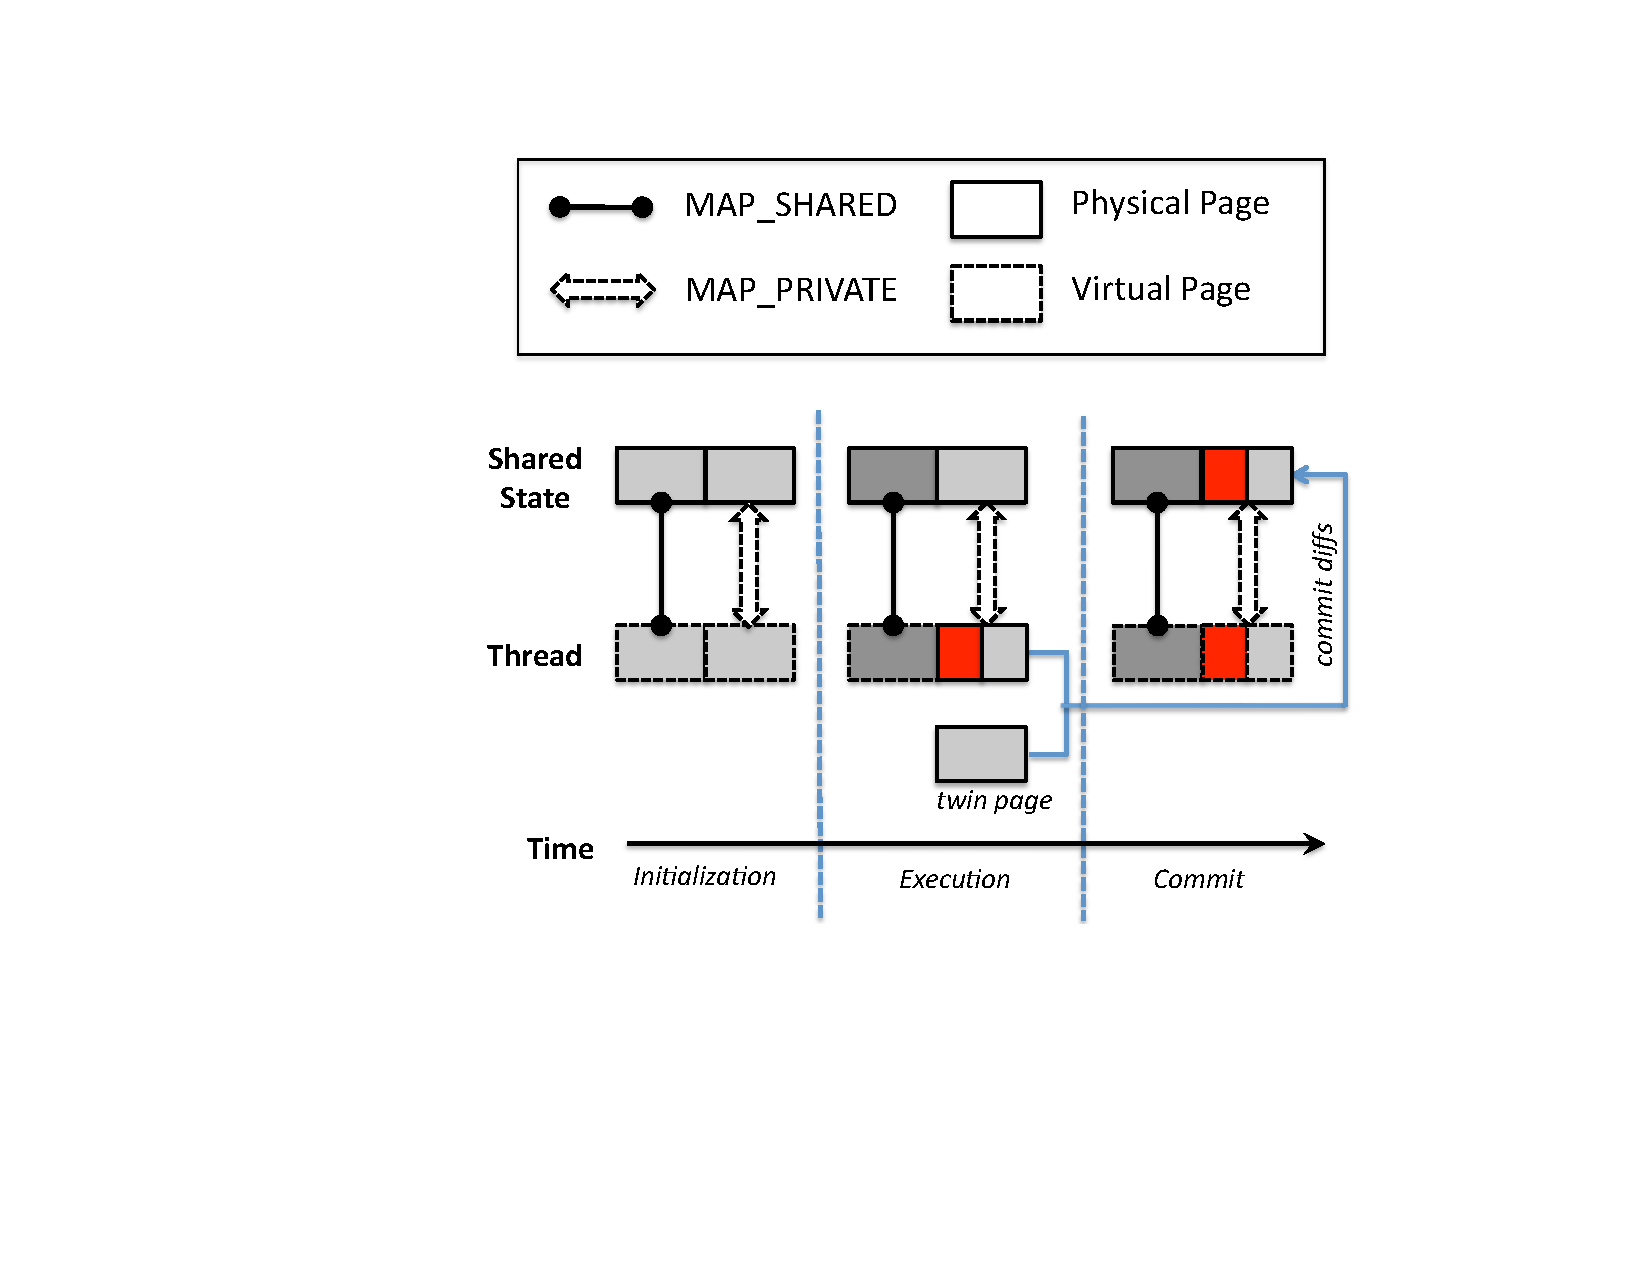
\includegraphics[width=3.5in]{figure/sheriffframework.pdf}
\caption{
\sheriff{} replaces \pthreads{} by simulating threads
with processes. It exposes an API that enables per-thread memory protection and memory isolation on a per-page basis. Each ``thread'' thus either operates directly
on shared memory, or on its own private
copy. For the latter, \sheriff{} commits diffs to shared mappings at synchronization
points (Section~\ref{simulation:syn}).
\label{fig:overview}}
\end{figure}

To create the effect of multi-threaded programs where
different threads share the same address space, \sheriff{} uses
memory mapped files to share the heap and globals across different
processes.  Note that \sheriff{} does not share the stack across
different processes because different threads have their own stacks
and, in general, multithreaded programs do not use the stack for cross-thread
communication.

\sheriff{} creates two different mappings for both the heap and the
globals.  One is a shared mapping, which is used to hold shared state.
The other is a private, copy-on-write (COW) per-process mapping that
each process works on directly.  Private mappings are linked to the
shared mapping through the one memory mapped file. Reads initially go
directly to the shared mapping, but after the first write operation,
both reads and writes are entirely private. \sheriff{}
updates the shared image at synchronization points, as described in
Section~\ref{simulation:thread}.

\sheriff{} uses a fixed-size mapping to hold
globals, which it checks to ensure is large enough to hold all
globals. \sheriff{} also uses a fixed-size mapping to store the heap
(by default, 1GB). Memory allocation requests from user
applications are satisfied from this fixed-size private mapping.

Since different threads allocate memory from this single fixed-size
mapping, the global superheap data structure is shared among different
threads and allocations are protected by one process-based mutex.  In
order to avoid false sharing induced by the memory allocator,
\sheriff{} employs a scalable ``per-thread'' heap organization that is
loosely based on Hoard~\cite{BergerMcKinleyBlumofeWilson:ASPLOS2000}
and built using HeapLayers~\cite{BergerZornMcKinley:2001}.  \sheriff{}
divides the heap into a fixed number of sub-heaps (currently 16).  The
metadata for each sub-heap is also shared by different threads and
protected by a cross-process mutex.  In order to reduce lock
contention, \sheriff{} assigns different sub-heaps to each thread at
creation time. Since each thread's heap allocates from different pages, 
the allocator itself is unlikely to collocate two objects from different 
threads on the same cache line.

Note that tools built with \sheriff{} can specify, on a per-page basis,
whether to use a shared mapping (so that updates are immediately
visible to other ``threads''), or a private mapping (so that updates
are delayed). Both \sheriffdetect{} and \sheriffprotect{} take
advantage of this facility.

\subsection{Shared File Access}
\label{sec:fileshare}

In multithreaded programs, all threads share the same file descriptor table
that tracks the process' open files.  For example, if one thread opens a 
file, the other threads see that the file has been opened.  However, 
multiple processes each have their own resources, including not only 
memory but also file handles, sockets, device handles, and windows.

While \sheriff{} could manage these directly, our current prototype
takes advantage of a feature of Linux that allows selective sharing of
memory and file descriptors. \sheriff{} sets the \texttt{CLONE\_FILES}
flag when creating new processes, resulting in child processes with
different address spaces but the same shared file descriptor table.

\subsection{Synchronization}
\label{simulation:syn}

\sheriff{} supports the full range of POSIX synchronization
operations (mutexes, conditional variables, barriers), as well as all
thread-related calls, including cancellation.

At each synchronization point, \sheriff{} must commit all changes made
by the current thread. The span between
synchronization points thus constitutes a single atomic
transaction. Note that \sheriff{}'s approach differs significantly
from previous transactional memory proposals~\cite{transaction},
including Grace. \sheriff{} is not optimistic, does not replace locks
with speculation (it actually acquires program-level locks), never
needs to roll back (it is always able to commit successfully), and
achieves low overhead for long transactions.

To simulate multithreaded synchronization, \sheriff{}
intercepts all synchronization object initialization function calls,
allocates new synchronization objects in a mapping shared
by all processes, and initializes them to be accessible by different
processes.

\sheriff{} wraps
all synchronization operations, including mutexes, condition
variables, and barriers in a similar fashion. For example, a call to
\texttt{pthread\_mutex\_lock} first ends the current transaction, 
then calls the corresponding \pthreads{} library function but on a
cross-process mutex. \sheriff{} then starts a new transaction after the
lock is acquired, which ends with the next synchronization operation.

Thread-related calls are implemented in terms of their process
counterparts. For example, \texttt{pthread\_join} ends the current
transaction and calls \texttt{waitpid} to wait for the appropriate
process to complete.


\subsection{Updating Shared Memory}

\label{sec:updatingsharedmemory}

At each synchronization point, \sheriff{} updates the shared
globals and heap with any updates that thread made.  To accomplish
this \sheriff{} uses \emph{twinning} and \emph{diffing}, mechanisms
first introduced in distributed shared memory systems to reduce
communication overhead~\cite{dsm:munin,dsm:treadmarks}.

% CC: Removed this, since diffs are always used to identify modifications
% \sheriffdetect{} uses diffs to identify modifications.

Figure~\ref{fig:overview} presents an overview of both mechanisms at
work. All private pages are
initially write-protected. Before any page is modified, \sheriff{}
copies its contents to a ``twin page'' and then unprotects the
page. At a synchronization point, \sheriff{} compares each twin page
to the modified page (byte by byte) to compute diffs.

\subsection{Example Execution}
\label{simulation:thread}

This section walks through an example of \sheriff{}'s execution from the start of a program to its termination.

% Figure~\ref{fig:overview} presents an overview of \sheriff{}'s execution.

\paragraph{Initialization: } Before the program begins, \sheriff{}
establishes the shared and local mappings for the heap and globals,
and initiates the first transaction.

\paragraph{Transaction Begin:}
At the beginning of every transaction, \sheriff{} write-protects any shared
pages so that later writes to these pages can be caught by
handling \texttt{SEGV} protection faults.  In later transactions,
\sheriff{} only write-protects pages dirtied in the last
transaction, since the others remain write-protected.

\paragraph{Execution: } While performing reads, \sheriff{} runs at
the same speed as a conventional multithreaded
program. However, the first write to a protected page triggers a page
fault that \sheriff{} handles.

\sheriff{} records the page holding the faulted address and then unprotects
this page so that future accesses run at
full speed.  Each page thus incurs at most one page fault per transaction.
Although protection faults and signals are expensive, these costs are
amortized over the entire transaction.

However, before servicing the fault, \sheriff{} must first obtain an
exact copy of this page (its twin). \sheriff{} accomplishes this by
forcing a copy-on-write operation on this page by writing to the start
of this page with contents from the same address (i.e., it
reads and writes the same value).

This step is essential to ensure that the twin is identical to the
original, unmodified page. After the signal handler, the OS's
copy-on-write mechanism creates a new, private page.

\paragraph{Transaction End: } At the end of each atomically-executed
region---at thread exit and before synchronization
points---\sheriff{} commits changes from
private pages to the shared space and reclaims memory holding old
private pages and twin pages.

\sheriff{} commits only the differences between the twin and the
modified pages. Once it has written these diffs, \sheriff{} issues an
\texttt{madvise} call with the \texttt{MADV\_DONTNEED} flag that
discards the physical pages backing both the private mapping and the
twin pages. This action allows the OS to reclaim this memory, helping
to ensure that \sheriff{}'s memory overhead remains close to that of
the original program.

\subsection{Discussion}

As Section~\ref{simulation:sharememory} notes, \sheriff{} does not
share the stack between different threads. When using \pthreads{},
threads are allowed to share stack variables with their parent.
As long as threads do not modify these variables,
\sheriff{} operates correctly. However, \sheriff{} does not preserve
\pthreads{} semantics for applications whose threads
\emph{modify} stack variables from their parent thread that their
parent then reads. Fortunately, passing stack variables to a thread
for modification is generally frowned upon, making it a rare coding
practice.

\sheriff{} cannot currently intercept atomic operations
written in assembly, so programs that implement their own
\emph{ad hoc} synchronization operations are not guaranteed to work
correctly (Xiong et al.\ have shown that 22--67\% of the uses of
\emph{ad hoc} synchronization they examined led to bugs or severe
performance issues~\cite{ad-hoc-considered-harmful}). We expect this
limitation to be less of a problem in the future because the
forthcoming C++0x standard exposes atomic operations in a standard
library, making it possible for \sheriff{} to intercept them.


\section{\sheriffdetect{}}


\begin{figure*}[!t]
\centering
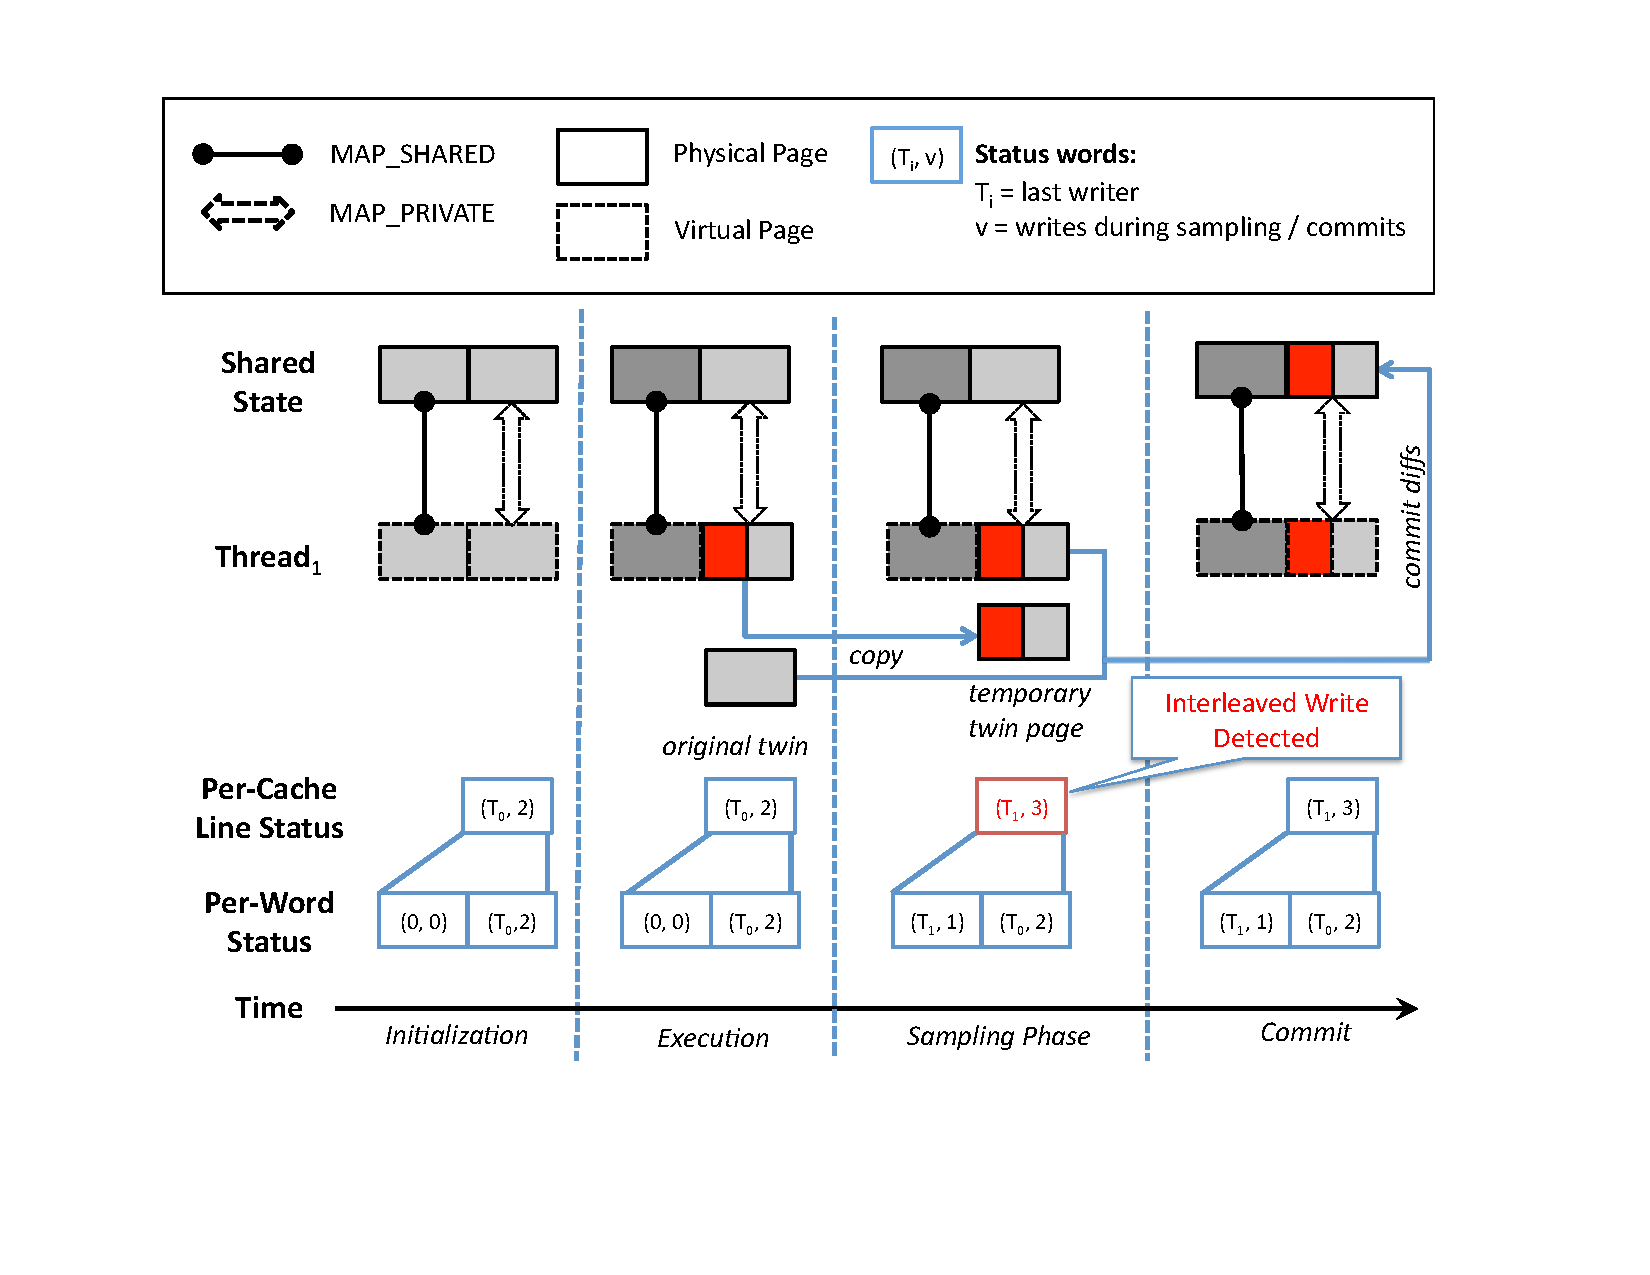
\includegraphics[width=6in]{figure/sheriffdetective}
\caption{
Overview of \sheriffdetect{}'s operation.
\sheriffdetect{} extends \sheriff{} with page ownership tracking, sampling,
and  \emph{per-cache line and per-word status} arrays
that track frequent false sharing
within cache lines. For clarity of exposition, the diagram depicts just one cache line per page and two words per cache line.
\label{fig:detectiveoverview}}
\end{figure*}

\label{sec:falseshare}

We use the \sheriff{} framework to build two
tools that address false sharing. This section
describes the first of these, \sheriffdetect{}, which detects false sharing.

\sheriffdetect{} detects both types of false sharing described in
the literature. The first is the sharing of structurally-unrelated
objects that happen to be located on the same cache line (i.e.,
different variables). The second is when multiple processors access
different fields of the same object, which Hyde and Fleisch describe
as ``pseudo sharing''~\cite{falseshare:Analysis}.

\sheriffdetect{} is designed to report only those instances of false sharing with
the potential to seriously degrade performance. False sharing
only causes a significant performance degradation when multiple threads
concurrently and repeatedly update falsely-shared data, leading to
large numbers of invalidation misses.

\subsection{Page Ownership Tracking}
\label{falseshare:basic mechanism}

One approach to implementing \sheriffdetect{} would be to use \sheriff{} and direct it to 
protect all pages and map them private.
The only change needed to detect false sharing would be an added check of twins
and diffs against committed pages. Any cache line whose contents
differ from the twin indicates it was changed by another thread. False sharing
has occurred whenever a diff (a
local update) lies on the same cache line as a local update.

However, this na\"{\i}ve approach would be quite costly. Since all local
modifications of different threads must be committed to the shared
space at every synchronization point to ensure correct
execution (see Section~\ref{simulation:syn}), this approach would
introduce substantial and unnecessary overhead for applications with a
large number of unshared pages.

To reduce this overhead, \sheriffdetect{} leverages a simple insight:
if two threads can falsely share a cache line, then
they must simultaneously access the page containing that
cache line.

Guided by this insight, \sheriffdetect{} relies on page protection to
gather information about whether pages are shared or not.
Instead of placing everything in the private address space,
\sheriffdetect{} utilizes its knowledge about page sharing patterns and
only maps those shared pages private.

\sheriffdetect{} initially read-protects all memory pages
and tracks the number of threads that attempt to write a page concurrently.
Any attempt to write to a
page will trigger a page fault.
\sheriffdetect{} then
increments the access counter for this page before unprotecting the page.
Once the access counter for a given page reaches two,
the page is considered to be shared,
and the page is mapped privately to each process to allow \sheriffdetect{} to locate possible false sharing.

% The protection can be done both in the periodic timer handler and at the end of one transaction.

\subsection{Discovering Local Modifications}
\label{falseshare:memorywrites}

When \sheriffdetect{} concludes each transaction, it compares each dirty page
with its twin a word at a time to find any modifications. \sheriffdetect{} thus
identifies all writes made by the current thread. 
Whenever local modifications are found, either in the sampling period or
at the end of a transaction (outside a critical section), \sheriffdetect{}
sets the virtual status words that indicate local modifications by the
current thread.

\subsection{Identifying Problematic False Sharing}
\label{detection:sampling}

\sheriffdetect{} uses sampling to measure the performance impact of
false sharing, which it uses to rank its reports.  \sheriffdetect{}
currently uses a sampling interval of 10 milliseconds, which we
empirically observe balances accuracy and performance overhead.

\sheriffdetect{} tracks the frequency of updates made to cache lines
by associating a temporary twin page with each private, modified page
(see Figure~{\ref{fig:detectiveoverview}}). These temporary twins are
created only during sampling, and are updated to reflect the current
working version at every sampling interval.

\label{detection:invalidation}

Only repeatedly interleaved writes (that is, by different threads) can
degrade performance by repeatedly forcing cache line
invalidations.  \sheriffdetect{} monitors interleaved writes across
different threads in order to capture this effect.

\sheriffdetect{} associates a \emph{per-cache line status} with
each cache line in every tracked page
(Figure~\ref{fig:overview}). This status contains two fields. The
first points to the last thread to write to this cache line, and the
second records the number of interleaved updates to the cache line.
Every time a different thread writes to a cache line, \sheriffdetect{}
updates the associated status word with both the thread id and the
version number. To reduce overhead, \sheriffdetect{} splits the
status into two different arrays to allow the use of atomic operations
instead of locks.

In addition, during sampling and at commit time, \sheriffdetect{}
updates \emph{per-word status} values for every modified word. This
information is later used to report the approximate frequency of
updates at the individual word granularity. Programmers can then use
this information to decide where to place padding. For example, if two
struct fields are falsely shared, padding should be placed
between the fields that are most frequently updated.

\sheriffdetect{} imposes relatively low memory overhead by maintaining
status values only for pages that are shared by multiple threads. To
further save space, \sheriffdetect{} stores each status in a single
32-bit word. The upper 16 bits stores the thread id, and the lower 16
bits stores the version number. When a word is detected to have been
modified by more than two threads, \sheriffdetect{} sets the thread id
field to \texttt{0xFFFF}, indicating that it is shared.

%  The \texttt{CacheInvalidation}
%array capture those interleaving cache invalidation for all
%cache lines in protected memory.  Every cache line has a corresponding
%counter to indicate the interleaving of cache invalidation for this
%cache line.  LastThreadModifyCache array is used to record last thread
%id to write on its cache line.


\subsection{Reporting}

\label{detection:object}

At this point, \sheriffdetect{} has detected individual cache lines that
are responsible for a large number of invalidations, and thus potential
sources of slowdowns. The next step is to identify the culprit objects.

\sheriffdetect{} aims to provide as much
context as possible about false sharing in order to reduce programmer
effort, identifying global variables by name, heap objects by
allocation context, and where possible, the fields modified by
different threads.
\sheriffdetect{} also provides an option to print out detailed information for every word in a
given cache line, including the number of updates and the accessor threads.

\sheriffdetect{} identifies globals directly by using debug
information that associates the address with the name of the
global. For heap objects, \sheriffdetect{} instruments memory
allocation to attach the call site to the header of each heap
object. This calling context indicates the sequence of function calls
that led to the actual allocation request, and is useful to help the
programmer identify and correct false sharing, as the case
study in Section~\ref{evaluation:comparison} demonstrates. Any heap
object responsible for a large number of invalidations is not
deallocated so that it can be reported at the end of program
execution.

\subsection{Avoiding False Positives}
\label{detection:avoidfalsepositive}

\sheriffdetect{} instruments memory allocation operations to
clean up cache invalidation counts whenever an object is
de-allocated. This approach avoids the false positives caused by
incorrectly aggregating counts when one address is re-used for other
objects.

\subsection{Reporting Falsely Shared Objects}

Once execution is complete, \sheriffdetect{} generates a ranked list of
falsely shared objects.  \sheriffdetect{} scans the cache invalidation
array for cache lines with a number of invalidations above a fixed
threshold (currently 100).  The corresponding invalidation times and
offset of this cache line are added to a global linked list sorted by
invalidation times.

After scanning the cache invalidation array, \sheriffdetect{} obtains object
information for all cache lines in the linked list, and reports
the allocation site and offsets of all falsely-shared allocated objects.

\subsection{Optimizations}

\sheriffdetect{} employs several optimizations that further reduce its overhead.

\paragraph{Reducing timer overhead.} 
As explained in Section~\ref{detection:sampling},
\sheriffdetect{} uses sampling to track 
interleaved writes by triggering a timer signal via \texttt{ualarm}. To reduce the
impact of timer interrupts, \sheriffdetect{} activates sampling
only when the average transaction time is larger than a threshold time
(currently 10 milliseconds). \sheriffdetect{} uses an exponential moving
average to track average transaction times ($\alpha = 0.9$). This
optimization does not significantly reduce 
the possibility of finding false sharing since
\sheriffdetect{}'s goal
 is to find an object with a large amount of interleaved
writes from different threads.

\paragraph{Sampling to find shared pages.} \sheriffdetect{} relies on
page protection to determine whether pages are shared or not. When one
application has a large number of transactions or page touches, the
protection overhead to gather this sharing information can dominate running
time.

\sheriffdetect{} reduces overhead by using sampling to detect shared
pages. If objects on a page are frequently falsely shared, the page
itself must also be frequently shared, so even relatively infrequent
sampling will eventually detect this sharing.  \sheriffdetect{}
currently samples the first 50 out of every 1,000 periods (one period
equals one transaction or one sampling interval). At the beginning of
each sampled period, all memory pages are made read-only so that any
writes to each page will be detected.  Once a page is found to be
shared, \sheriffdetect{} will track any false sharing inside it.
\sheriffdetect{} only updates the shared status of pages during
sampled periods and at commit points. During unsampled periods, pages
whose sharing status is unknown impose no protection overhead.

\subsection{Discussion}

Unlike previous tools, \sheriffdetect{} has no false positives, differentiates true sharing from
false sharing, and avoid false positives caused by the reuse of heap objects.
\sheriffdetect{} can under-report false sharing instances in the following situations:

\paragraph{Single writer.}
False sharing usually involves updates from multiple threads, but it
can also arise when there is exactly one thread writing to part of a
cache line while other threads read from it. Because its detection
algorithm depends on multiple, differing updates, \sheriffdetect{} cannot
detect this kind of false sharing.

\paragraph{Heap-induced false sharing.}  \sheriff{} replaces the standard
memory allocator with one that behaves like Hoard and thus reduces the
risk of heap-induced false sharing. \sheriffdetect{} therefore does
not detect false sharing caused by the standard memory allocator.
Since it is straightforward to deploy Hoard or a similar allocator
to avoid heap-induced false sharing, this limitation is not a problem
in practice.

%Besides, using some Hoard-like memory allocator can be very helpful to improve the performance of multi-threaded programs
%and that should be the standard for memory allocator for multi-threaded programs.

\paragraph{Misses due to sampling.}  Since it uses sampling to
  capture continuous writes from different threads, \sheriffdetect{} can
  miss writes that occur in the middle of sampling intervals. We
  hypothesize that false sharing instances that affect performance are
  unlikely to perform frequent writes exclusively during that time, and so
  are unlikely to be missed.


\section{\sheriffprotect{}}
\label{sec:patrol}

While \sheriffdetect{} can be effective at locating the sources of
false sharing, it is sometimes difficult or impossible for programmers
to remove the false sharing that \sheriffdetect{} can reveal. For
instance, padding data structures to eliminate false sharing within an
object or different elements of an array can cause excessive memory
consumption or degrade cache utilization~\cite{zhao:vee:2011}. Time
constraints may prevent programmers from investing in other solutions,
or the source code may simply be unavailable. \sheriffprotect{}, our
second tool developed with the \sheriff{} framework, can take
unaltered C/C++ binaries and eliminate the performance degradation
caused by false sharing.

To accomplish its goals, \sheriffprotect{} relies on a key insight
due initially to DuBois et al.\
~\cite{Dubois:1991:DCE:125826.125941}: \emph{delaying updates avoids
  false sharing.}  Delaying one thread's updates
so that they do not cause invalidations to other threads 
eliminates the performance impact of false sharing. Consider the case when
two threads are updating two falsely-shared objects A and B. If one
thread's accesses to A were delayed so that they preceded all of the
other thread's accesses to B, then the false sharing would cause no
invalidations and hence have no performance impact.

In effect, this is exactly what \sheriff{} does already when all pages
are mapped private. By using processes instead of threads, all updates
between synchronization points are applied to different physical addresses
belonging to the different ``threads''. In this way, \sheriff{} itself
prevents false sharing by not updating the same physical cache
lines.

However, using \sheriff{} with all pages mapped private would be impractical as a runtime
replacement for \pthreads{}, because it would impose excessive overhead.
This overhead arises due to 
protection and copying costs that would counteract the benefit of
preventing false sharing.

For example, when a thread updates a large number of pages between
transactions, \sheriff{} must commit all local changes to the shared
mapping at the end of every transaction, \emph{even in the absence of
  sharing}. The associated protection and copying overhead can
dramatically degrade performance. The same problem arises when transactions are
short (e.g., when there are frequent lock acquisitions), because the
cost of protection and page faults cannot be amortized by the
protection-free part of the transaction.

\sheriffprotect{} implements two key optimizations that improve performance by directly addressing these issues.

\paragraph{Focus on smaller objects:}
  \sheriffprotect{} focuses its false sharing prevention exclusively
  on small objects (those less than 1024 bytes in size). All large
  objects are mapped shared and are never protected. 

  First, we expect small objects to be a likely source of false
  sharing because they fit on a cache line. False sharing in large
  objects like arrays is also possible, but we expect the amount of
  false sharing relative to the size of the object to be far lower
  than with small objects (an intuition that \sheriffdetect{}
  confirms, at least across our benchmark suite). For such objects,
  the cost of protection would outweigh the advantages of
  preventing false sharing.

  Second, the total amount of memory consumed by small objects tends
  to be less than that consumed by large objects. Because the cost of
  protecting and committing changes is proportional to the volume of
  updates, \sheriffprotect{} limits protection to small objects,
  reducing overhead while capturing the benefit of false sharing
  prevention where it matters most.

\begin{table*}[!t]
\centering
\begin{tabular}{l|c|c|c}
\hline
{\bf \small Microbenchmark} & {\bf \small Performance-Sensitive /} & {\bf \small \sheriffdetect{} } & {\bf \small PTU } \\
 & {\bf \small Actual False Sharing?} & & \\
\hline

\small {\em False sharing (adjacent objects)} & Yes & $\checkmark$ & $\checkmark$\\
\small {\em Pseudo sharing (array elements)} & Yes & $\checkmark$ & $\checkmark$\\
\hline
\small {\em True sharing} & No &  & \\
\small {\em Non-interleaved false sharing} & No  & & $\times$\\
\small {\em Heap reuse (no sharing)} & No & & $\times$\\
\hline
\end{tabular}
\caption{False sharing detection results using PTU and \sheriffdetect{}. 
\sheriffdetect{}
correctly reports only actual false sharing instances, and only those with a
performance impact; $\checkmark$ denotes a correct report, and
$\times$ indicates a spurious report (a false positive).
\label{table:microbenchmarks}}
\end{table*}


\paragraph{Adaptive false sharing prevention:} 
  Short transactions do not give \sheriff{} the chance to amortize its
  protection overheads. To address this, \sheriffprotect{} employs a simple adaptive
  mechanism.  \sheriffprotect{} tracks the
  length of each transaction and uses exponential weighted averaging
  ($\alpha = 0.9$) to calculate the average transaction length.  Once
  the average transaction length is shorter than an established
  threshold, \sheriffprotect{} switches to using shared mappings for
  all memory and does no further page protection. As long as
  transactions remain too short for \sheriffprotect{} to have any
  benefit, all of its overhead-producing mechanisms remain switched
  off. If the average transaction length rises back above the
  threshold, \sheriffprotect{} re-establishes private mappings and
  page protection.



%\section{Discussion}
%\label{sec:discussion}

This section analyzes some key limitations of \dthreads{} that
restrict its ability to run certain programs, limit the extent of
determinism it can guarantee, or potentially affect performance.

%\dthreads{} is a fully deterministic multithreaded system, which ensures a deterministic order of 
%both synchronization operations and all memory accesses. The most close
%work to us is CoreDet~\cite{Bergan:2010:CCR:1736020.1736029}.


\textbf{Unsupported programs: }
\dthreads{} currently does not support programs with ad hoc
synchronization that avoids the \pthreads{} library, such as those
that use atomic operations implemented in assembly.  However, the
upcoming C++0X standard includes a library interface for atomic
operations~\cite[pp. 1107--1128]{c++0xstandarddraft}, and a future
version of \dthreads{} could correctly implement these by intercepting
these library calls and treating them as synchronization points. While
ad hoc synchronization is a common practice, it is also a notorious
source of bugs; Xiong et al.\ show that 22--67\% of the uses of ad hoc
synchronization lead to bugs or severe performance
issues~\cite{ad-hoc-considered-harmful}.

\dthreads{} also currently does not write-share the stack
across threads, so that updates made by a thread to a stack variable
would not be reflected back to the parent, which could cause a program
to fail. Passing stack variables to a thread for modification is
extremely error-prone and generally deprecated, making this a rare
coding practice.

\textbf{External determinism: }
While \dthreads{} provides internal non-determinism, it does not
guarantee determinism when a program's behavior depends on external
sources of non-determinism, such as system time or I/O
events. Incorporation of \dthreads{} in the dOS framework, an OS
proposal that enforces system-level determinism, would provide full
deterministic execution, although this remains future
work~\cite{deterministic-process-groups}.

\textbf{Runtime performance: }
Section~\ref{sec:evaluation} shows that \dthreads{} can provide high
performance for a number of applications; in fact, for the majority of
the benchmarks examined, \dthreads{} matches or even exceeds the
performance of \pthreads{}. However, \dthreads{} does occasionally
degrade performance, sometimes substantially. The primary culprit is
the intensive use of locks (that is, when programs that acquire and
release locks at high frequency), which are much more expensive
in \dthreads{} than in \pthreads{}. The \texttt{ferret} benchmark from
the PARSEC benchmark suite exemplfies this behavior.

However, programmers using \dthreads{} could greatly reduce the use of
locks, and thus improve performance, by taking advantage
of \dthreads{}' strong isolation guarantee between threads.


%  Since Surprise locking inside libraries. Not a limitation \emph{per
%  se} but definitely an issue that could surprise programmers.

% Draft can be downloaded from http://www.open-std.org/jtc1/sc22/wg21/docs/papers/2010/n3126.pdf.
%Fine once they are library calls, as they are in gcc and in the upcoming C++0X standard (cite!), since then we can intercept them.

\textbf{Memory consumption: }
Finally, because \dthreads{} creates private, per-process copies of
modified pages between commits, it can increase a program's memory
footprint by the number of modified pages between synchronization
operations. This increased footprint does not seem to be a problem in
practice, both because the number of modified pages is generally far
smaller than the number of pages read, and because it is transitory:
all private pages are relinquished to the operating system
(via \munmap{}) at the end of every commit operation.

%Increased memory footprint (linear in the number of dirtied (modified) pages).




\section{Evaluation}
\label{sec:evaluation}

All evaluations are performed on a quiescent Intel Core 2 dual-processor system equipped with 
16GB of RAM. 
%whereas each processor has 4 cores. 
%processor with 4 cores), with 8GB of RAM. 
Each processor is a 4-core 64-bit Intel Xeon running at 2.33 GHz with a 4MB
shared L2 cache and 32KB private L1 cache. 
The underlying operating system is unmodified CentOS 5.5, running with Linux kernel
version 2.6.18-194.17.1.el5. The glibc version is 2.5. 
In order to compare the performance fairly, all benchmarks were built as 64-bit executables 
using LLVM compiler (version 3.2). The compiler optimization level is set to ``-O1'' 
so memory allocation callsites can be reported precisely.
%since we can not report line number of source code with optimization level larger than
%``-O2''.
In our evaluation, we choose two popular benchmark suites, Phoenix~\cite{phoenix-hpca} and PARSEC~\cite{parsec}.

Our evaluations aim to answer the following questions:
\begin{itemize}
\item
  How effective is \defaults{} on detecting and predicting false sharing problem (Section ~\ref{sec:effective})?

\item
  What is the performance overhead of \defaults{} with and without prediction
  (Section ~\ref{sec:perfoverhead})?

\item
  What is the memory overhead of \defaults{}~ (Section~\ref{sec:memoverhead})?
\end{itemize}


\subsection{Detection and Prediction Effectiveness}
\label{sec:effective}

\subsubsection{Benchmarks}
To compare with state-of-the-art false sharing detection work~\cite{sheriff, OSdetection}, 
we also executes \defaults{} on two existing benchmark suites 
suites Phoenix~\cite{phoenix-hpca} and PARSEC~\cite{parsec}, 
and results are listed in the Table~\ref{table:detection}. 

%Our results show that \defaults{} not only capture previously-discovered
%false sharing, but also many detect new false sharing places. The results
%are listed in Table~\ref{table:detection}. 

%http://www.technovelty.org/tips/getting-a-tick-in-latex.html
%http://tex.stackexchange.com/questions/42619/x-mark-to-match-checkmark
%\begin{comment}
\begin{table*}[ht!]
{
\centering
\begin{tabular}{l|r|r|r}
\hline
{\bf \small Benchmark} & {\bf \small Source Code} & {\bf \small New} & {\bf \small Improvement} \\
%{\bf \small Benchmark} & {\bf \small Source Code} & {\bf \small Type of False Sharing} & {New} & {\bf \small Improvement} \\
\hline
\small \textbf{histogram} & {\small histogram-pthread.c:213} & \cmark{} & 46.22\%\\
\small \textbf{reverse\_index} & {\small reverseindex-pthread.c:511} & \xmark{} & 0.09\%\\
\small \textbf{word\_count} & {\small word\_count-pthread.c:136} & \xmark{} & 0.14\%\\
\hline
\small \textbf{streamcluster} & {\small streamcluster.cpp:985} & \xmark{} & 7.52\% \\
\small \textbf{streamcluster} & {\small streamcluster.cpp:1907} & \cmark{} & 4.77\%\\
%\small \textbf{bodytrack} & {\small TrackingModel.cpp:59} & 0 & \cmark{} & \\
\hline
\hline
\small \textbf{linear\_regression} & {\small linear\_regression-pthread.c:133} & \xmark{} & 1206.93\%\\
\hline
\end{tabular}
\caption{Detection results of \defaults{} on Phoenix and PARSEC benchmark suites. \label{table:detection}}
}
\end{table*}

In this table, the first column lists those programs with false sharing problems. 
The second column shows precisely where the problem is. Actually, all false sharing found
are internal object false sharing on heap objects, although \defaults{} has no 
problem to find intern-objects and global false sharing. So the memory allocation site 
are listed in the table.
The third column ``New'' marks whether this false sharing is newly found by \defaults{} or not.
False sharing found by previous work are marked as cross mark(\xmark{}) and those 
newly found false sharing are identified using a tick mark(\cmark{}). 
The last column ``Improvement'' shows the performance improvement after fixing false sharing 
based on the average result with $10$ runs. 
The improvement rate is calculated by substracting $1$ from normalized runtime. Taking 
\texttt{histogram} for an example here, original runtime of \texttt{histogram} is $0.75s$
and new runtime is $0.51s$, then the performance improvement is $(0.75/0.51) - 1$.

Seen from the table, \defaults{} reveals several unknown false sharing problems. \defaults{} detects 
false sharing in \texttt{histogram} and additional false sharing in line 1908 of
\texttt{streamcluster}. 
In \texttt{histogram}, multiple threads repeatedly modify different locations of the same heap object. 
Padding the data structure \texttt{thread\_arg\_t} fixes the false sharing problem and 
helps to improve the performance around 46\%.
In \texttt{streamcluster}, multiple threads are changing a \texttt{bool} array, \texttt{switch\_membership}, simultaneously. By simply changing this array to \texttt{long} type contributes to about 4.7\% performance improvement. 
%None of these two false sharing problems has been reported by previous tools.

Other false sharing problems has been revealed by previous tool \sheriff{}~\cite{sheriff}. 
Same as \sheriff{}, we didn't see much performance improvement for \texttt{reverse\_index} and 
\texttt{word\_count} since number of updates inside them is not a significant number. But they
are actually false sharing problems that have been verified manually by us.

\texttt{streamcluster} has another false sharing problem that different threads 
may change the same object simultaneously. 
Actually authors of \texttt{streamclsuter} have already realized possible
false shairing problems and meant to utilize a macro \texttt{CACHE\_LINE} to avoid it. Unfortunately,
the defaulted value of this macro is setted to $32$ bytes, which is different with the actual
cache line size that we are using. By setting to $64$ bytes instead, we see around $7.5\%$ performance
improvement.

linear\_regression has a significant false sharing problem. 
Different threads simultaneously changed an array of thread-indexed structures in a tight
loop, which causes a huge amount of cache invalidations. 
Fixing false sharing inside can improve the performance for $12\times$. 
Actually, if we do not enable prediction then 
we can not detect false sharing problem inside because false sharing behavior is 
very sensitive to the starting address of false sharing object. 
We are going to explore this more detailed in Section~\ref{sec:predicteval}.
Since \defaults{} are using a customized memory manager, which may
bring us different allocation metadata and different memory map for allocation,
false sharing problem may not manifest with ``-O1'' optmization flag of \texttt{clang}.
%http://tex.stackexchange.com/questions/42619/x-mark-to-match-checkmark
%\begin{comment}

\subsubsection{Real Applications}
To verify its practicability, we further evaluate \defaults{} 
on several widely-used real applications, which none of previous work has considered.  
These real applications include a server application \texttt{MySQL}~\cite{mysql}, 
a common C++ library \texttt{boost}~\cite{libfalsesharing} 
and a distributed memory object caching system \texttt{memcached}, a network retriver \texttt{aget}, 
a parallel bzip2 file compressor \texttt{pbzip2} and a parallel file scanner \texttt{pfscan}.
Among them, \texttt{MySQL} and \texttt{boost} are known to have some false sharing problem inside 
so we evaluate their specific versions, \texttt{MySQL-5.5.32} and
\texttt{boost-1.49.0}.

False sharing in \texttt{MySQL} has caused significant scalability problem and
it was very difficult to be identified. 
According to the architect of \texttt{MySQL} Mikael Ronstrom, ``we had gathered specialists on 
InnoDB..., participants from MySQL support... and a number of generic specialists on 
computer performance...'', ''the fruit of the meeting ... were able to 
improve \texttt{MySQL} performance by 6$\times$ with those scalability fixes''. 
The false sharing of boost library is caused by the special usage of \texttt{spinlock} pool and fixing
it brings 40\% performance improvement. 
\defaults{} is able to succesfully detect false sharing locations
in \texttt{MySQL} and \texttt{boost} library. 
For the other four applications, \defaults{} doest not find serere false sharing problems.

\subsubsection{Prediction Effectiveness}
\label{sec:predicteval}
We evaluates the prediction effectiveness of \defaults{} on the \texttt{linear\_regression} benchmark.
We choose this benchmark for two reasons:
\begin{enumerate}
\item
False sharing problem of this benchmark can not be detected without prediction. 

\item
This benchmark has a severe performance problem when false sharing actually occurs, which should be 
detected but can be omitted by exiting tools.
\end{enumerate}

The data structure of false sharing object and the source code
to experience false sharing is showed in Figure~\ref{fig:linearregression}. 
When we are using \texttt{clang} compiler while compiling for $64$bit binary, the size of this 
data structure is $64$ bytes.

\begin{figure}[!h]
{\centering
\subfigure{\lstinputlisting[numbers=none,frame=none,boxpos=t]{fig/linearregression.psedocode}}
\caption{False sharing problem inside \texttt{linear\_regression} benchmark.
\label{fig:linearregression}}
}
\end{figure}

For this false sharing problem, the main thread allocates an array of $8$ elements 
(if $8$ cores totally), 
with each element being a \texttt{lreg\_args} type. 
Then this array will be passed to different threads so that they can only updates its 
thread-dependent area, see Figure~\ref{fig:linearregression}.
Actually, different fields of this data structure \texttt{lreg\_args} has different access pattern:
only those fields between $SX$ and $SXY$ (totally around $40$ bytes) are constantly read and updated.

Thus, \texttt{linear\_regression} actually is very sensitive to the starting address 
of the false sharing object, which can be caused by many of dynamic properties 
listed in Section~\ref{sec:intro}, e.g.,
hardware platform, optimization flag, compiler etc.
This sensitivity can be seen in Figure~\ref{fig:perfsensitive}.
That is, when offset is $0$ or $56$ bytes, there is no false sharing at all.
Actually, using our customized memory manager,
the offset between the starting address of potential false sharing object 
and starting of cache line is actually $56$ bytes,
that explain why we can not detect false sharing problem without prediction enabled.

\defaults{} can predict false sharing problem precisely for all of these cases. This explains
the effectiveness of prediction tool.

\subsection{Performance Overhead}
\label{sec:perfoverhead}
To avoid the effect caused by extreme outliers,
all performance data are based on the average of 10 runs excluding the
maximum and minimum values.
Actual performance overhead can be seen in the following figure~\ref{fig:perf}. 

\begin{figure*}[!ht]
\begin{center}
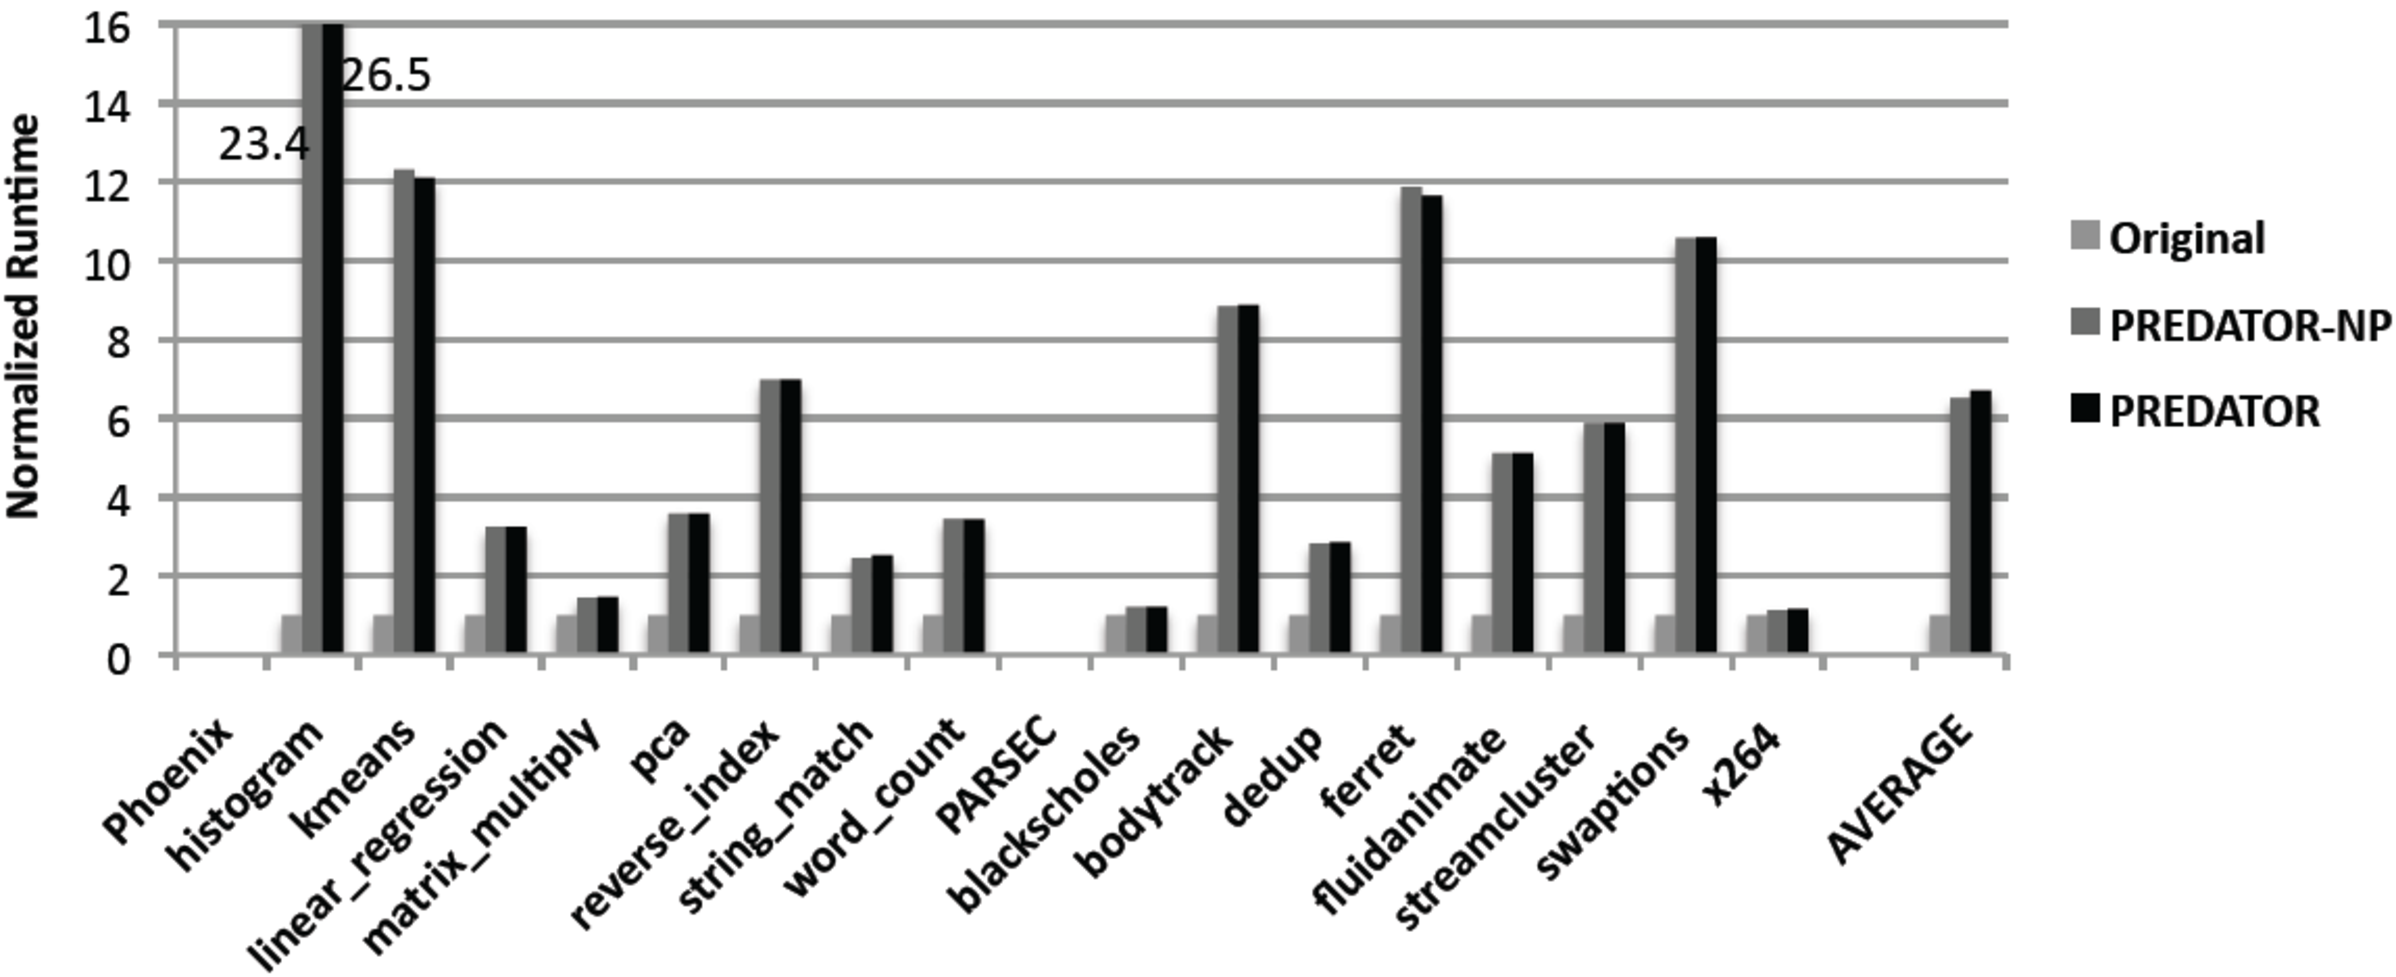
\includegraphics[width=5in]{fig/perf}
\end{center}
\caption{
Performance overhead of \defaults{} with and without prediction.
\label{fig:perf}}
\end{figure*}

Manifestness of false sharing highly depends on 

\subsection{Memory Overhead}
\label{sec:memoverhead}
Since \defaults{} pre-allocates a huge block of memory using \texttt{mmap} system call for 
its heap usage, 
virtual memory can not be used to tell actual memory overhead imposed by our tool. 
Hence, we only evaluate the physical memory overhead used by an application only. 
This number is based on proportional set size (PSS) in \texttt{/proc/self/smaps}
as discussed by Justin et al. ~\cite{memusage}. 

When evaluating an application, we start a script program to save 
corresponding \texttt{smaps} files periodically. 
The maximum number of total physical memory usage is selected for calculation.
%It is noted that we remove the physical memory usage of   
Results of memory usage is shown in Figure~\ref{fig:memusage}. As we can see,
\defaults{} does not increase memory usage substantially in all cases except for \texttt{swaptions}. 
Specifically, removing \texttt{swaptions} from calculation reduces 
the average memory overhead from 64\% to 22\%. 

The reason of \texttt{swaptions} using a large amount of memory is that 
its original memory usage is too small (only 3KB), and 
the additional memory added by \defaults{} in detection, prediction and
reporting yields a large number in percentage calculation. 

\begin{figure*}
\begin{center} 
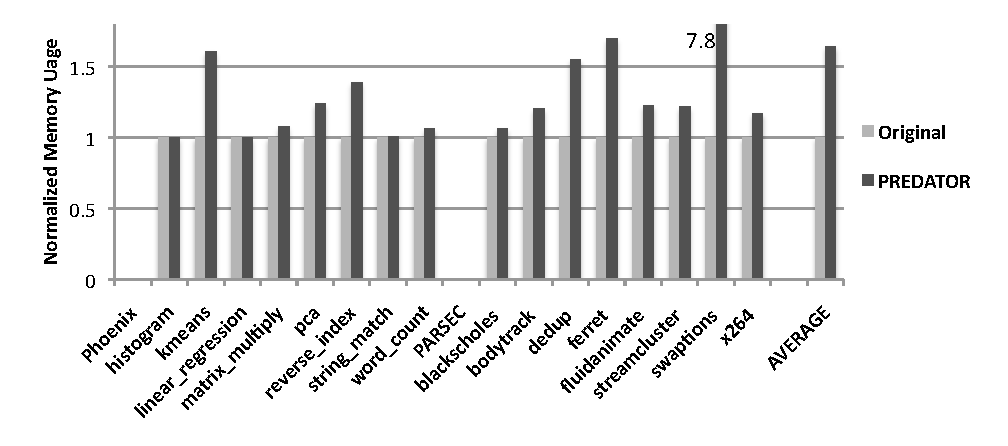
\includegraphics[width=5in]{fig/memusage}
\end{center}
%\includegraphics{fig/potential.pdf}
\caption{Memory usage overhead}
\label{fig:memusage}
\end{figure*}




%\section{Future Work}
%\label{sec:future}
\label{futurework}

We plan to extend \sheriff{} to find more performance related problems in
multithreaded programs. For example, if one frequently-read word
happens to be in the same cache line with one frequently-written word,
it would be better to separate those two words. But in the current
framework, \sheriff{} cannot detect a single memory read operation using the
twin page mechanism. We are examining the combination of hardware
watchpoints to help us locate this kind of performance error. In
addition, we plan to exploit watchpoints to capture those program
counters that touch specific addresses so as to point the programmer
to specific lines of code responsible for false sharing.




\section{Conclusion}
This paper introduces \emph{evidence-based dynamic analysis}, a new
lightweight dynamic analysis technique. Evidence-based dynamic
analysis works for errors that can be forced to leave evidence of
their presence. These errors include key problems for C and C++
programs: buffer overflows, dangling-pointer errors, and memory
leaks. Evidence-based dynamic analysis is fast because it lets the
application run at full speed until an error is detected; execution is
then rolled back and replayed with instrumentation at the point where
the evidence was found, pinpointing the error. We
present \doubletake{}, the first evidence-based dynamic analysis
framework, and implement these analyses inside it. The resulting
analyses are the fastest versions to date, demonstrating the
effectiveness and efficiency of this new dynamic analysis approach.
\doubletake{} is available for download at \url{http://github.com/plasma-umass/DoubleTake}.



\section{Acknowledgments}
The authors thank Luis Ceze and Charlie Curtsinger for their valuable
feedback and suggestions which helped improve this paper. We
acknowledge the support of the Gigascale Systems Research Center, one
of six research centers funded under the Focus Center Research Program
(FCRP), a Semiconductor Research Corporation entity.  This material is
based upon work supported by Intel, Microsoft Research, and the
National Science Foundation under CCF-0910883. Any opinions, findings,
and conclusions or recommendations expressed in this material are
those of the author(s) and do not necessarily reflect the views of the
National Science Foundation.

% \newpage

{
\bibliographystyle{abbrv}
\bibliography{ref,emery}
}

\end{document}
